% (The MIT License)
%
% Copyright (c) 2023-2024 Yegor Bugayenko
%
% Permission is hereby granted, free of charge, to any person obtaining a copy
% of this software and associated documentation files (the 'Software'), to deal
% in the Software without restriction, including without limitation the rights
% to use, copy, modify, merge, publish, distribute, sublicense, and/or sell
% copies of the Software, and to permit persons to whom the Software is
% furnished to do so, subject to the following conditions:
%
% The above copyright notice and this permission notice shall be included in all
% copies or substantial portions of the Software.
%
% THE SOFTWARE IS PROVIDED 'AS IS', WITHOUT WARRANTY OF ANY KIND, EXPRESS OR
% IMPLIED, INCLUDING BUT NOT LIMITED TO THE WARRANTIES OF MERCHANTABILITY,
% FITNESS FOR A PARTICULAR PURPOSE AND NONINFRINGEMENT. IN NO EVENT SHALL THE
% AUTHORS OR COPYRIGHT HOLDERS BE LIABLE FOR ANY CLAIM, DAMAGES OR OTHER
% LIABILITY, WHETHER IN AN ACTION OF CONTRACT, TORT OR OTHERWISE, ARISING FROM,
% OUT OF OR IN CONNECTION WITH THE SOFTWARE OR THE USE OR OTHER DEALINGS IN THE
% SOFTWARE.

\documentclass{article}
\usepackage{../sqm}
\newcommand*\thetitle{Code Style}
\begin{document}

\plush{\sqmTitlePage{22}{}}

\qte
  [Brian Kernighan]
  {../19-comments-density/brian-kernighan.jpg}
  {The harder it is for people to \ul{grasp the intent} of any given section, the longer it will be before the program becomes \ul{operational}. Trying to outsmart a compiler defeats much of the purpose of using one. Write clearly --- \ul{don't sacrifice} clarity for `efficiency.'}
  {kernighan1974elements}

\pptBanner{Which One Is Better?}
\begin{multicols}{2}
{\small\begin{ffcode}
int f(int n)
{
  if (n == 1 || n < 2)
    return 1;
  int r = f (n-1);
  int r2 = f(n - 2);
  return r +r2;
  }
\end{ffcode}
}
\par\columnbreak\par
{\small\begin{ffcode}
int fibonacci(int n) {
  if (n <= 2) {
    return 1;
  }
  return fibonacci(n - 1)
    + fibonacci(n - 2);
}
\end{ffcode}
}
\end{multicols}
\plush{}

\qte
  [Henry Ledgard]
  {henry-ledgard.jpg}
  {An individual's body language helps clarify the spoken word. In a similar sense, the programmer relies on \ul{white space}---what is not said directly---in the code to communicate logic, intent, and understanding.}
  {green2011coding}

\pitch{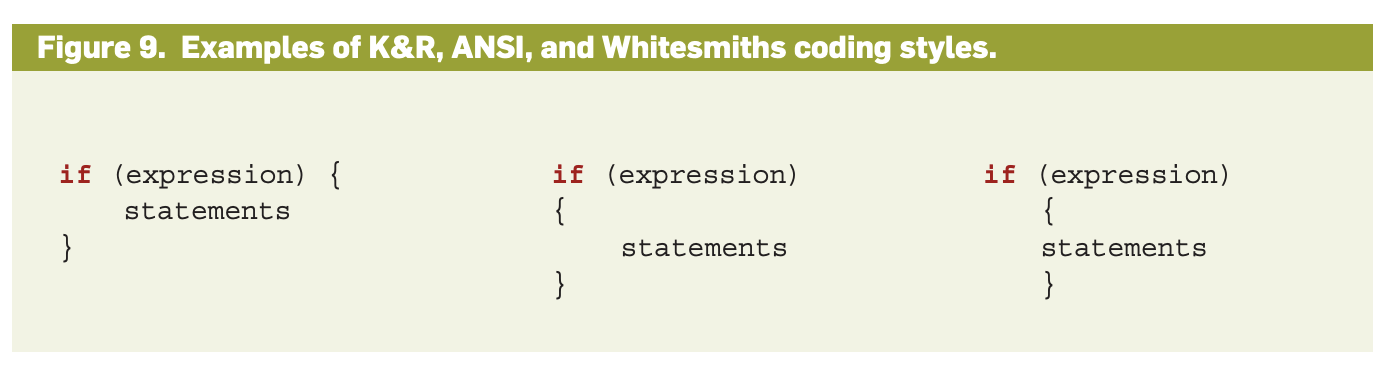
\includegraphics[width=.95\linewidth]{three-ifs.png}
  \source{green2011coding}}

\plush{\pptBanner{My Favorite Style Checkers}
  \begin{itemize}
    \item \href{https://www.qulice.com}{Qulice} for Java (\href{https://checkstyle.sourceforge.io/}{Checkstyle} + \href{https://pmd.github.io/}{PMD})
    \item \href{https://eslint.org/}{ESLint} for JavaScript
    \item \href{https://clang.llvm.org/extra/clang-tidy/}{Clang-Tidy} for C++
    \item \href{https://github.com/pylint-dev/pylint}{Pylint} for Python
    \item \href{https://github.com/rubocop/rubocop}{Rubocop} for Ruby
    \item \href{https://github.com/squizlabs/PHP_CodeSniffer}{PHP\_CodeSniffer} for PHP
    \item \href{https://github.com/rust-lang/rustfmt}{rustfmt} for Rust
  \end{itemize}}

\plush{\pptBanner{How Many Rules in Style Checkers?}
  \begin{itemize}
    \item 690+ in Clang-Tidy (C++)
    \item 550+ in Rubocop (Ruby)
    \item 400+ in PMD (Java)
    \item 130+ in Checkstyle (Java)
    \item 120+ in Pylint (Python)
  \end{itemize}
  \par{\small Some/most of the rules no only check style, but also find bugs\par}}

\plush{\pptBanner{Some Exotic Style Checkers}
  \begin{itemize}
    \item \href{https://github.com/koalaman/shellcheck}{Shellcheck} for Bash
    \item \href{https://github.com/markdownlint/markdownlint}{markdownlint} for Markdown
    \item \href{https://github.com/mrtazz/checkmake}{Checkmake} for Makefile
    \item \href{https://github.com/yegor256/xcop}{xcop} for XML
  \end{itemize}}

\end{document}
